\begin{frame}{Analyse des concordances des termes médicaux}
	Analyses effectuées dans \textsc{TXM}.
	\begin{itemize}
		\item on utilise un terme dans le contexte où on cite Charcot
		\begin{itemize}
			\item terme traditionnel (ex. \textit{paralysie agitante})
			\item synonyme ou terme relevant du champ conceptuel en question
			\begin{itemize}
%				\item ensembles de mots liés à un certain concept \citep{costachescu2024}\\
				\item \textit{pied tabétique} $\rightarrow$ forme particulière d'\textit{arthropathies tabétiques}
			\end{itemize}
		\end{itemize}
	\end{itemize}
	\begin{block}{Exemple}
		\texttt{([word = "paralysie"] [word = "agitante"] []* [word = "Charcot"] | [word = "Charcot"] []* [word = "paralysie"] [word = "agitante"]) within p}
		\begin{itemize}
			\item repérer toutes les occurrences dans un paragraphe où \textit{paralysie agitante} et \textit{Charcot} apparaissent dans n'importe quel ordre, séparés par 0 ou plusieurs mots
		\end{itemize}
	\end{block}
\end{frame}

\begin{frame}{Références à Charcot}
	
	\begin{table}
		\centering
		\resizebox{\textwidth}{!}{%
			\begin{tabular}{|l|p{10cm}|}
				\hline
				\textbf{Terme} & \textbf{Contexte} \\
				\hline
				\textit{maladie de Parkinson} & [$\dots$] \underline{paralysie agitante} que \textbf{Charcot} a eu raison de dénommer \underline{maladie de Parkinson} \\
				\hline
				\textit{ataxie locomotrice progressive} & [$\dots$] arthropathies [$\dots$] de l'\underline{ataxie locomotrice}, [$\dots$] signalées, pour la première fois, par M. \textbf{Charcot}. \\
				& [$\dots$] \underline{ataxie locomotrice progressive}, constatée par douze médecins, parmi lesquels, [$\dots$] MM. \textbf{Charcot} [$\dots$] \\
				\hline
				\textit{arthropathies tabétiques} & [$\dots$] mais personne n'avait encore décrit des cas d'\underline{arthropathie tabétique}, lorsque, en 1808, M. le professeur \textbf{Charcot} publia la première observation d'arthropathie chez un ataxique.\\
				\hline
				\textit{trépidation épileptoïde du pied} & [$\dots$] \underline{trépidation}, qui se propage parfois à tous les \underline{membres}. Ce spasme, [$\dots$] peut entraîner à sa suite des rétractions fibro-tendineuses analogues à celles que \textbf{Charcot} a décrites chez l'homme, [$\dots$] \\
				\hline
				\textit{sclérose en plaques disséminées} & [$\dots$] une combinaison de la \underline{sclérose en plaques}, bien décrite déjà par \textbf{Charcot} et Vulpian [$\dots$] \\
				\hline
			\end{tabular}
		}
		\caption{Concordance des termes médicaux faisant référence à Charcot -- corpus Autres.}
	\end{table}
\end{frame}


\begin{frame}{Références à Charcot}
	
	\begin{table}
		\centering
		\resizebox{\textwidth}{!}{%
			\begin{tabular}{|l|p{10cm}|}
				\hline
				\textbf{Terme} & \textbf{Contexte} \\
				\hline
				\textit{tremblement} & [$\dots$] \textbf{Charcot} présentait, dans son amphithéâtre, pour démontrer les caractères oscillatoires des diverses variétés de \underline{tremblements}. \\
				\hline
				\textit{nystagmus} & SCLÉROSE EN PLAQUES [$\dots$] [$\dots$], \underline{nystagmus}, [$\dots$]. La difficulté de la résoudre est d'autant plus grande qu'à côté des foyers de sclérose en plaques avec tous les caractères histologiques classiques décrits depuis \textbf{Charcot}, il y a des foyers avec une
				destruction plus ou moins complète des cylindraxes [$\dots$]\\
				\hline
				\textit{embarras parole} & Lorsqu'on se trouve en présence d'un malade ayant de l'\underline{embarras de la parole} [$\dots$] A. La réponse à la première proposition n'est nullement embarrassante, si l'on veut se rappeler ces paroles de M. le professeur \textbf{Charcot} : [$\dots$] \\
				\hline
				\textit{sclérose latérale amyotrophique} & [$\dots$] \underline{sclérose latérale amyotrophique}, maladie découverte par mon illustre maître \textbf{Charcot}. \\
				\hline
				\textit{tics convulsifs} & désignée par M. \textbf{Charcot} sous le nom de maladie des \underline{tics convulsifs} \\
				\hline
				\textit{atrophie musculaire progressive} & \textbf{Charcot} et Marie ont décrit la \og{}forme particulière d'\underline{atrophie musculaire progressive}\fg{}\\
				\hline
				\textit{aphasie} & Lorsqu'il y a, dit M. le professeur \textbf{Charcot} (1), suppression de la mémoire pour l'articulation des mots, c'est l'\underline{aphasie} motrice d'articulation ou \underline{aphasie} de Broca qui se présente.\\
				\hline
			\end{tabular}
		}
		\caption{Concordance des termes médicaux faisant référence à Charcot -- corpus Autres (suite).}
	\end{table}
\end{frame}

\begin{frame}{Références à Charcot}
	
	\begin{table}
		\centering
		\resizebox{\textwidth}{!}{%
			\begin{tabular}{|l|p{10cm}|}
				\hline
				\textbf{Terme} & \textbf{Contexte} \\
				\hline
				\textit{astasie-abasie} & [$\dots$] forme particulière d'impuissance motrice dont M. P. Blocqe a donné la
				définition suivante \og{}[$\dots$], et qu'il a désigné sous le nom expressif d'\underline{astasie} et d'\underline{abasie}. C'est là un état morbide sur lequel M. le professeur \textbf{Charcot} est	fréquemment revenu dans ses Leçons du mardi [$\dots$]\\
				\hline
				\textit{athétose} & symptôme désigné par M. W. Hammond sous le nom d'\underline{athétose} [$\dots$] M. \textbf{Charcot} a fait remarquer que cette définition était imparfaite pour les motifs suivants : [$\dots$] \\
				\hline
				\textit{chorées} & \underline{Chorée} hystérique ou rhythmique. C'est à M. le professeur \textbf{Charcot} que nous devons une exacte description de cet état pathologique. \\
				\hline
				\textit{hystérie} & C'est encore à \textbf{lui} [Charcot] que nous devons la connaissance de l'\underline{hystérie} traumatique [$\dots$] \\
				\hline
				\textit{épilepsie} & M. \textbf{Charcot} a décrit avec le plus grand soin l'\underline{épilepsie} partielle d'origine syphilitique [$\dots$] \\
				\hline
				\textit{hypnose} & Les trois états de l'\underline{hypnose} décrits par M. \textbf{Charcot} sont devenus classiques, [$\dots$] \\
				\hline
				\textit{systématisation de l'organisation de la moëlle épinière} & \underline{systématisation de la moelle}, synthèses [$\dots$]. Mais \textbf{Charcot}, on l'a vu, est, par nature, enclin à la synthèse. \\
				\hline
				\textit{localisations cérébrales} & Je vous ai montré \textbf{Charcot}, concourant pour
				la plus grosse part, à l'édification de la doctrine des \underline{localisations cérébrales}, qui est devenue quelque chose comme la préface d'une psychologie nouvelle.\\
				\hline
			\end{tabular}
		}
		\caption{Concordance des termes médicaux faisant référence à Charcot -- corpus Autres (fin).}
	\end{table}
\end{frame}

\begin{frame}{Analyse des cooccurrences}
	\begin{itemize}
		\item quels cooccurrents avec les termes médicaux ciblés ? 
		\begin{itemize}
			\item Charcot, Babinski, Necker$\dots$
		\end{itemize}
		\item recensement des résultats pour le cooccurrent : Charcot
		\item sinon, autre cooccurrent (médecin) avec l'indice le plus élevé\\
		\begin{alertblock}{Exemple}
			\texttt{[word = "athétose"]} 
			\begin{itemize}
				\item liste des cooccurrents pour le terme \textit{athétose}
			\end{itemize}
		\end{alertblock}
	\end{itemize}
\end{frame}

\begin{frame}{Analyse des cooccurrences}
	\begin{table}[h]
		\centering
		\resizebox{\textwidth}{!}{%
			\begin{tabular}{rrrrrr}
				\textbf{Terme} & \textbf{Cooccurrent} & \textbf{Fréquence} & \textbf{Co-fréquence} & \textbf{Indice} & \textbf{Distance moyenne} \\
				\hline
				maladie de Parkinson  & Charcot & 2 968 &  3 & 2 & 3,3\\
				ataxie locomotrice progressive  & Charcot & 2 968 & 3 & 2 & 5,3 \\
				arthropathies tabétiques & Charcot & 2 968 & 4 & 5 & 1,5 \\
				trépidation épileptoïde du pied & Babinski $\cdot$ Charcot &  1 134 &  8 & 12 & 4,8 \\
				sclérose en plaques disséminées & Charcot & 2 968 & 7 & 3 & 6,3 \\
				tremblement & Achard & 137 & 3 & 2 &  2,3\\
				nystagmus & Barany & 11 & 3 & 7 & 3,3\\
				embarras parole & Chervin & 41 & 8 & 17 & 4,5\\
				sclérose latérale amyotrophique & Charcot & 2 968 & 4 & 3 & 3,5 \\
				tics convulsifs & Charcot & 2 968 & 6 & 8 & 5,2 \\
				atrophie musculaire progressive & Charcot & 2 968 & 4 & 3 & 6,0 \\
				aphasie & Charcot & 2 968 & 7 & 2 & 4,0\\
				astasie-abasie & Charcot & 2 968 & 2 & 2 & 1,5 \\
				athétose & Hammond & 34 & 2 & 4 & 1,5\\
				chorées & Sydenham & 129 & 63 & 163 & 1,1 \\
				\rowcolor{yellow!30}hystérie & Charcot & 2 968 & 52 & 19 & 5,4\\
				épilepsie & Jackson & 52 & 34 & 78 & 0,2 \\
				hypnose & Braid & 567 & 14 & 12 & 4,7 \\
				systématisation de l'organisation de la moëlle épinière & NA & NA & NA & NA & NA \\
				localisations cérébrales & Charcot & 2 968 & 9 & 7 & 5,3 \\
			\end{tabular}
		}
		\caption{Analyse des cooccurrences des termes médicaux à partir du corpus Autres.}
		\label{tab:cooccurrences}
	\end{table}
	
\end{frame}

\begin{frame}{Analyse des cooccurrences}
	Absence occasionnelle de cooccurrent Charcot expliquable :
	\begin{itemize}
		\item \textit{épilepsie} : terme créé par J. H. Jackson
		\item \textit{hypnose} : terme créé par J. Braid
		\item \textit{athétose} : terme créé par W. A. Hammond
		\item \textit{chorées} : définition moderne par T. Sydenham
		\item \textit{trépidation épileptoïde du pied} : Babinski ? Vulpian? Charcot ? 			
	\end{itemize}
\end{frame}

\begin{frame}{Analyse des autres cooccurrents}
	\begin{table}
		\centering
		\resizebox{\textwidth}{!}{%
			\begin{tabular}{|l|p{10cm}|}
				\hline
				\textbf{Terme} & \textbf{Contexte} \\
				\hline
				\textit{trépidation épileptoïde du pied} (\textit{clonus}) & \textbf{On} [Babinski] le désigne alors sous la dénomination de \og{}\underline{clonus du
					pied}\fg{}, \og{}\underline{trépidation épileptoïde du pied}\fg{} \\ \hline
				\textit{tremblement} &  D'après \textbf{Charcot} et surtout d'après \textbf{Achard}, ce \underline{tremblement} aurait de certaines analogies avec le tremblement sénile, [$\dots$] \\ \hline
				\textit{nystagmus} & [$\dots$] les recherches inspirées par les
				travaux de \textbf{Barany} sur le \underline{nystagmus} provoqué indiqueraient une certaine fréquence de troubles labyrinthiques [$\dots$] \\ \hline
				\textit{embarras parole} & M. le Dc \textbf{Chervin}, [$\dots$] vient de rédiger un nouveau résumé des notions cliniques fondamentales indispensables à connaître sur quelques \underline{troubles fonctionnels de la parole} et notamment sur le bégaiement. 
				\\
				\hline
				\textit{athétose} & [$\dots$] nous avons affaire au symptôme désigné par M. W. \textbf{Hammond} sous le nom d'\underline{athétose}.\\
				\hline
				\textit{chorées} & Cependant, la \underline{chorée} de \textbf{Sydenham} présente quelques particularités sémiologiques que nous allons passer en revue.\\ \hline 
				
				épilepsie & Depuis les remarquables travaux de M. Hughlings \textbf{Jackson} sur la forme d'\underline{épilepsie} à laquelle il a attaché son nom, [$\dots$] \\ \hline
				\textit{hypnose} & Selon \textbf{Braid}, l'\underline{hypnose} est caractérisée par des phénomènes mentaux et physiques, particuliers à cette condition.\\
				\hline
			\end{tabular}
		}
		\caption{Concordance des termes médicaux faisant référence à d'autres médecins -- corpus Autres.}
	\end{table}
\end{frame}

%\begin{frame}{Cas ambigu de la \textit{trépidation épileptoïde du pied} (\textit{clonus})}
%	
%	\begin{quote}
%		\textbf{On} le désigne alors sous la dénomination de \og{}\underline{clonus du pied}\fg{}, de \og{}\underline{trépidation épileptoïde du pied}\fg{}.
%	\end{quote}
%	\begin{flushright}
%		\small
%		\parencite{babinski1934oeuvre}
%	\end{flushright}
%	
%	
%	
%	\begin{quote}
%		\small
%		[$\dots$] l'un d'eux, [$\dots$], est
%		connu en France sous le nom de \underline{trépidation provoquée},	\underline{d'épilepsie spinale provoquée}. Les auteurs allemands rappelent le phénomène du pied ‭{\underline{Fussph\oe{}nomen}}, ou encore le \underline{clonus du pied}.
%		Mais c'est là un signe qui appartient ‭à la clinique française. Dès ‭1863, [$\dots$], il ‭était journellement mis ‭à profit dans les services de la Salpêtrière, par M. \textbf{Vulpian}, par \textbf{moi-même} et par \textbf{nos ‭élèves}.
%	\end{quote}
%	
%	\begin{flushright}
%		\small
%		\parencite{brissaud1893}
%	\end{flushright}
%	%		CL\_000001\_004 (pas inclus dans le corpus Autres -.-)
%	%		\bigskip
%	%					\begin{quote}
%		%			“$\dots$ known in France under the name of \underline{provoked trepidation}, or \underline{provoked spinal epilepsy}. German writers call it the foot-phenomenon (\underline{Fussphoenomen}) or \underline{ankle clonus}. But \textbf{the discovery of this sign belongs to French clinical observers}. Since 1863$\dots$ it has been \textbf{practised} daily in the wards of La Salpêtrière \textbf{by M. Vulpian, by myself} {\normalfont[Charcot]}, \textbf{and by our pupils}.”
%		%		\end{quote}
%	%		\begin{flushright}
%		%			\small
%		%			\citep{charcot1883lectures}
%		%		\end{flushright}
%	%	
%\end{frame}

%\begin{frame}{Analyse comparative des approches employées}
%	\begin{itemize}
	%		\item \textit{PatternRank} valorise systématiquement les termes
	%		\item pas de consensus entre les métriques
	%		\begin{itemize}
		%			\item l'écart le plus petit entre eux : \textit{hypnose}
		%		\end{itemize}
	%	\end{itemize}
%\begin{figure}[h]
%	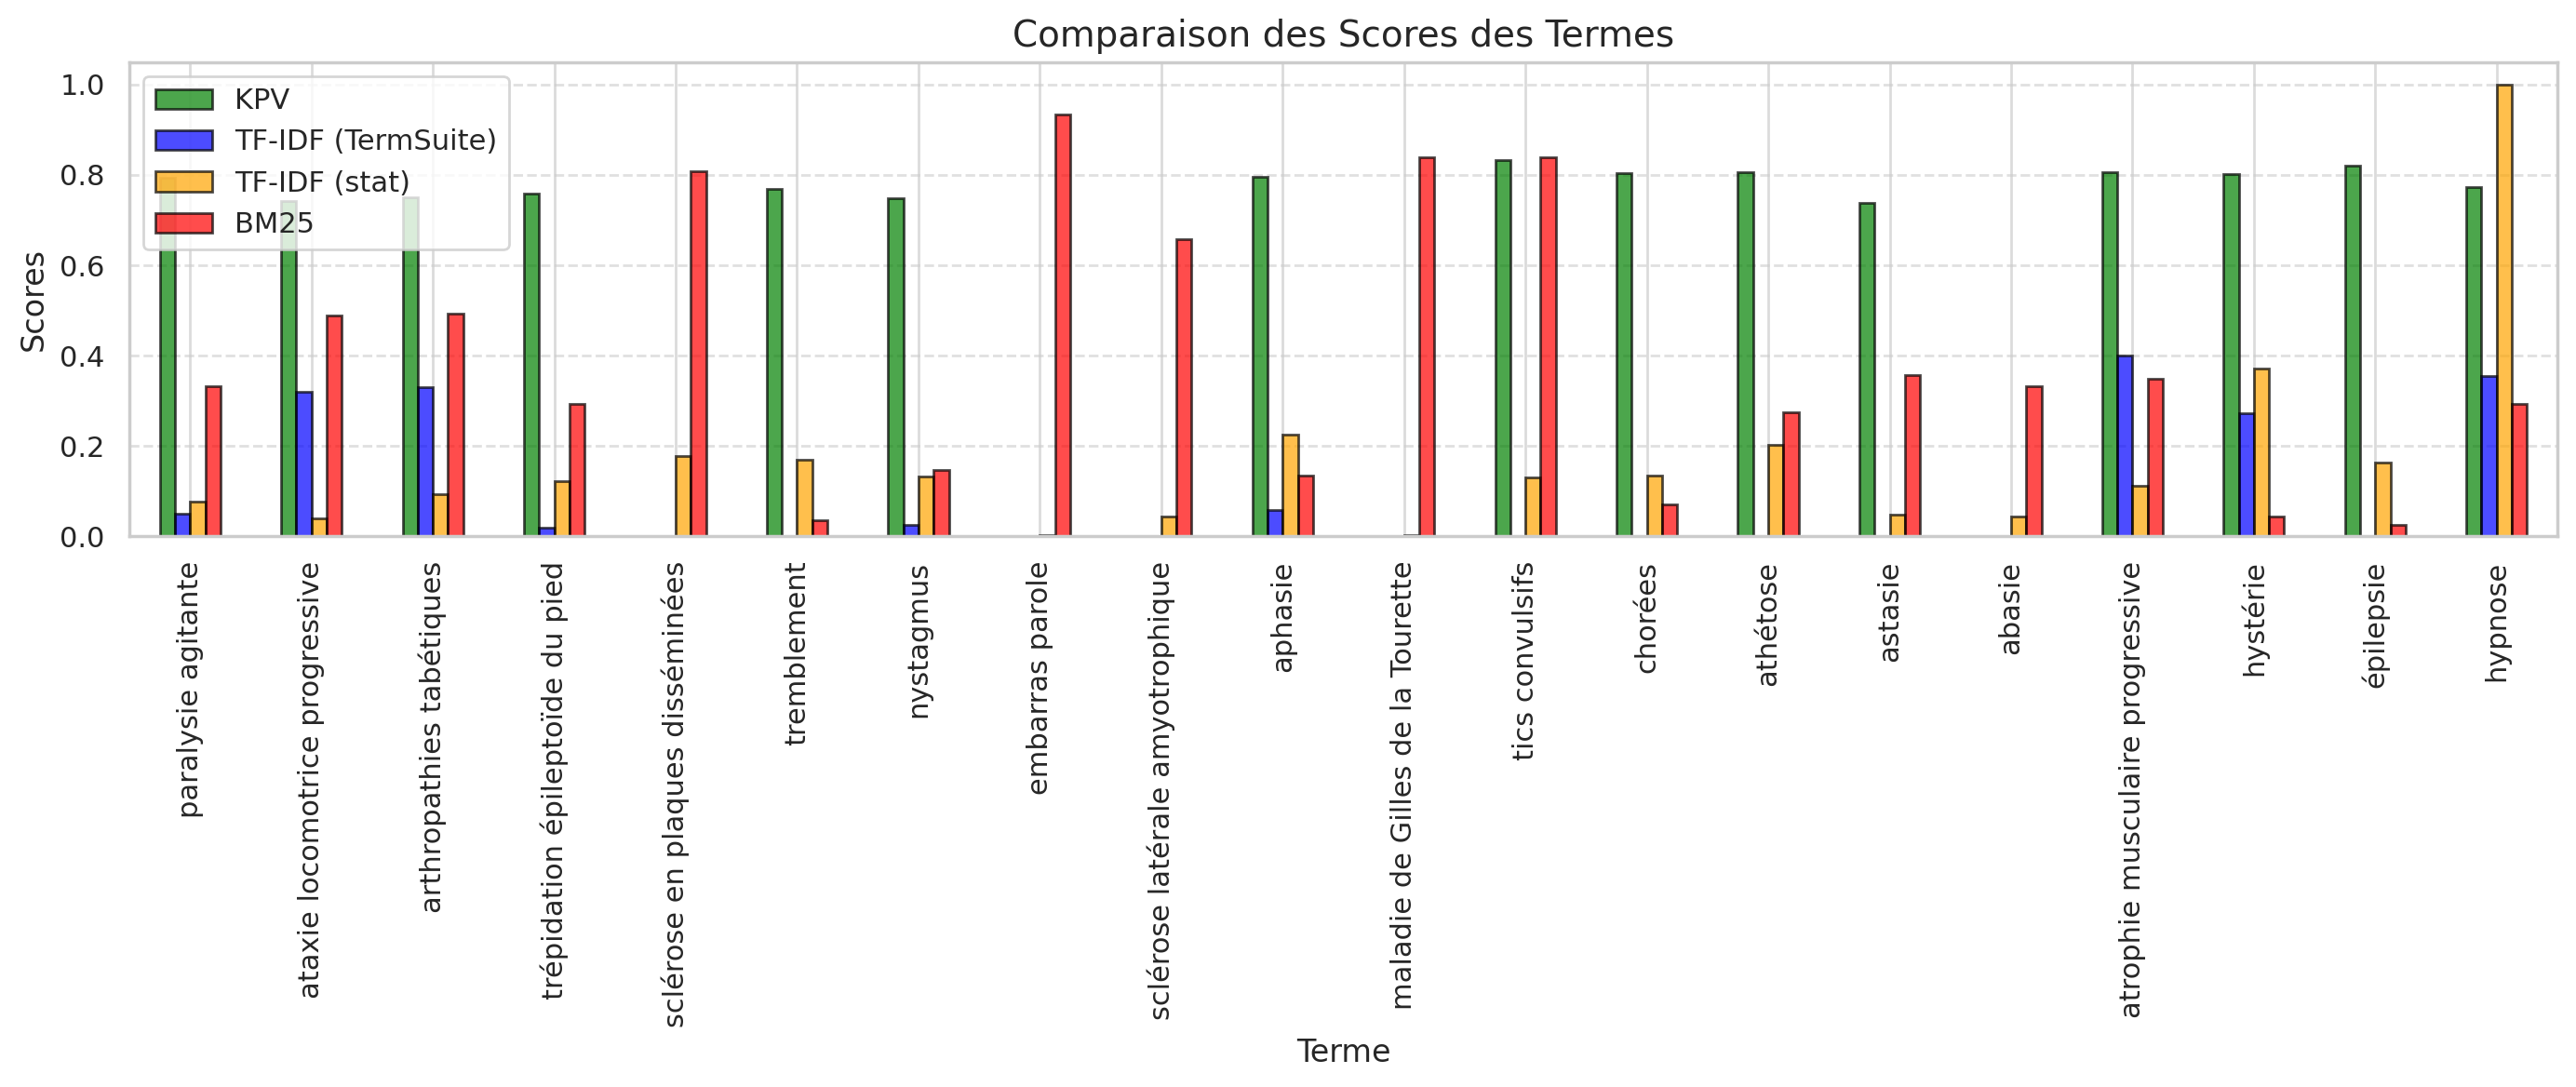
\includegraphics[width=\linewidth]{pic/termes_viz.png}
%	\caption{Visualisation des scores de pertinences pour chaque terme de référence}
%	\label{fig:ling_out_TAL}
%\end{figure}
%\end{frame}

%\begin{frame}{\textit{PatternRank}}
%	Les termes les plus pertinents dans \og{}Autres\fg{} :
%\begin{table}[h]
%	\centering
%	\begin{tabular}{|l|l|c|}
	%		\hline
	%		\textbf{Terme} & \textbf{Synonyme} & \textbf{Score} \\
	%		\hline
	%		\texttt{tics convulsifs} & \bolder{syndrome de Tourette} & \textsc{0.8331} \\
	%		\texttt{état parkinsonien} & \bolder{maladie de Parkinson} & 0.7936 \\
	%%		\texttt{paralytiques agitants} & \bolder{maladie de Parkinson} & 0.7851 \\
	%		\hline
	%	\end{tabular}
%\end{table}
%\end{frame}





%\begin{frame}{Chronologie d'une locution : indice de croissance de l'impact ?}
%\begin{figure}[h] % Use [H] to force the figure to stay in place
%	\begin{itemize}
	%		\item évolution de la fréquence des termes au sein des deux corpus\footnote{\url{https://obtic.huma-num.fr/obvie/charcot/?view=corpus}}
	%		\item convergence entre des termes : fin \textsc{XIX}\ieme{}, début \textsc{XX}\ieme{} s.
	%%		\begin{itemize}
		%%				\item \textit{ppm} : nombre d’occurrences par million de mots 
		%%		\end{itemize}
	%	\end{itemize}
%	\centering
%	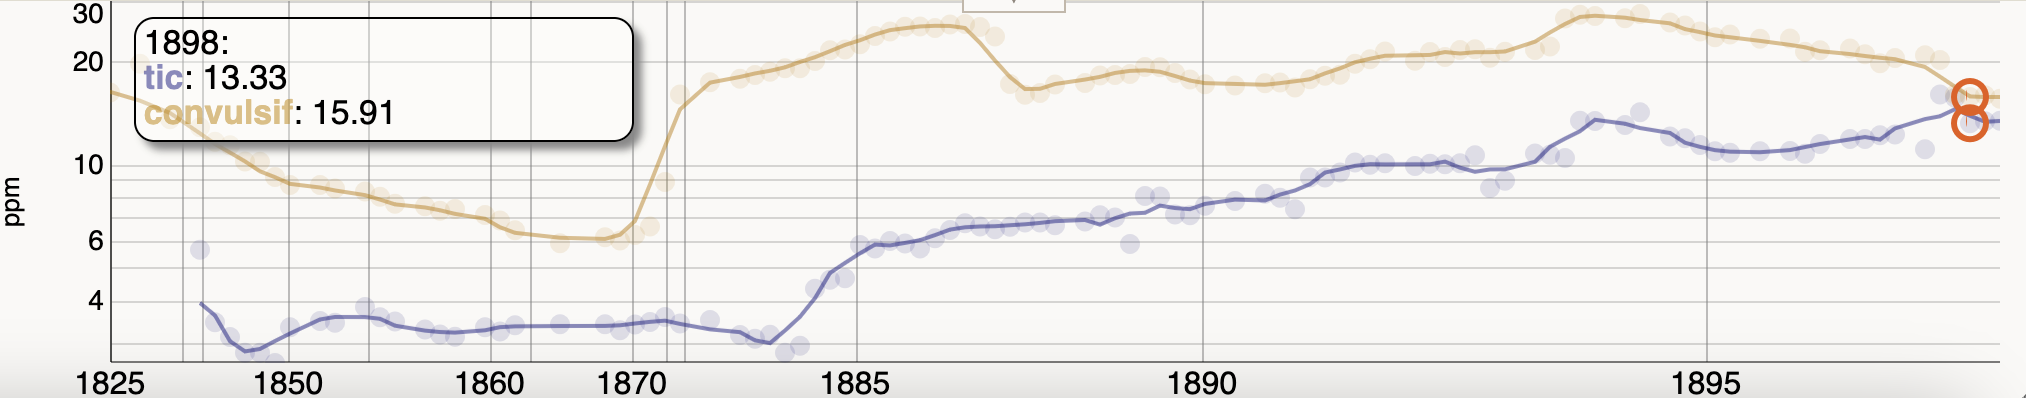
\includegraphics[width=\linewidth]{pic/tics_convulsifs.png}
%	\caption{Chronologie de la fréquence du terme \textit{tic convulsif}.}
%	\label{fig:ling_out_TAL}
%\end{figure}
%
%\begin{figure}[h]
%	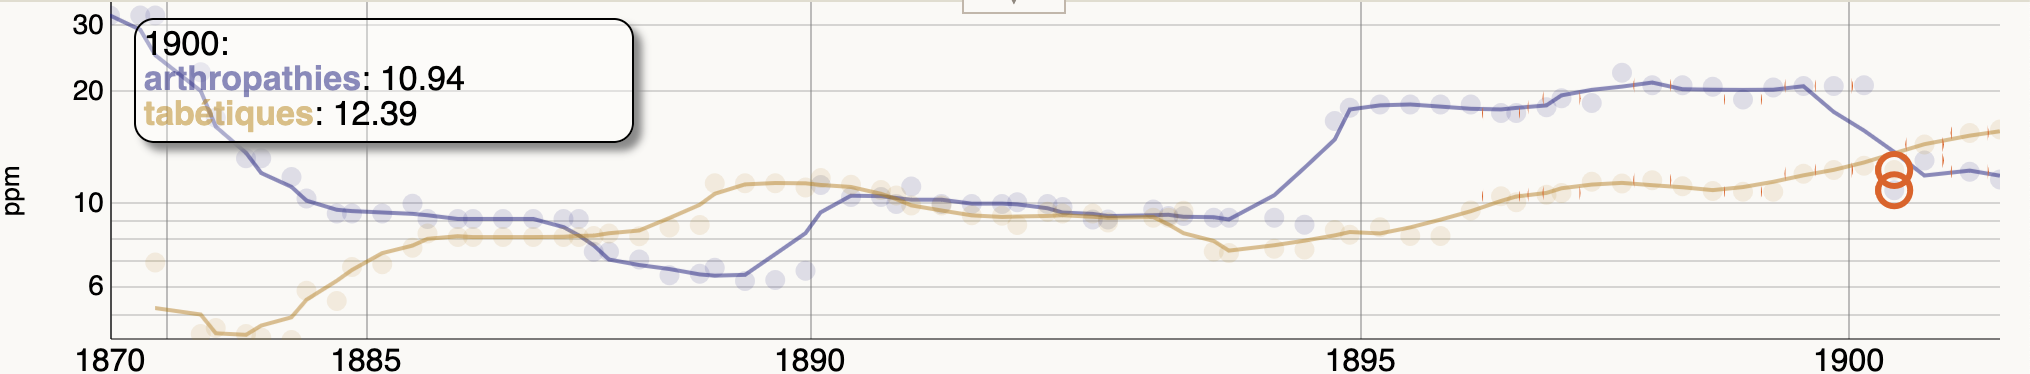
\includegraphics[width=\linewidth]{pic/arthropathies_tabetiques.png}
%\caption{Chronologie de la fréquence du terme \textit{arthropathies tabétiques}.}
%\label{fig:ling_out_TAL}
%\end{figure}
%\end{frame}
